%%%%%%%%%%%%%%%%%%%%%%%%%%%%%%%%%%%%%%%%%%%%%%%%%
%
%	MSc THESIS TEMPLATE
%	developed for my master thesis at the Universitá di Torino
%
%	by Eugenio Senes (eugenio.senes@gmail.com)
%
%	released under MIT license, so share, modify and enjoy, but quoting the author !
%
%%%%%%%%%%%%%%%%%%%%%%%%%%%%%%%%%%%%%%%%%%%%%%%%%


%% DOCUMENT CLASS (alternative to book is 'report')
% Print just right page or both sides (comment the other one)
\documentclass[12pt,a4paper,openright,oneside]{report}	%%One sided
%\documentclass[12pt,a4paper,openright,twoside]{book}	%%Double sided


%% SET MARGINS OF THE PAGES
\usepackage{geometry}
\geometry{a4paper,portrait, left=35mm, right=30mm, top=35mm, bottom=30mm}

%% HEADERS AND FOOTERS
\usepackage{fancyhdr}
\pagestyle{fancy}
\fancyhf{} 			%clears default header and footer
\rhead{} 			%right head
\lhead{ \leftmark} 	%left head
\rfoot{\thepage}
%%consider using also chead, cfoot, lfoot
%coherce the plain stile to this (e.g. the first page of every chapter)
\fancypagestyle{plain}{
	\fancyhf{}
	\rfoot{\thepage}
	\renewcommand{\headrulewidth}{0pt}
	\renewcommand{\footrulewidth}{0pt}
}
%% CLEAR PAGE WITHOUT NUMBER AT THE BEGINNING OF CHAPTERS
\let\origdoublepage\cleardoublepage
\newcommand{\clearemptydoublepage}{%
  \clearpage
  {\pagestyle{empty}\origdoublepage}%
}
%% ALLOW PAGE ROTATION
\usepackage{lscape}

%% HYPERTEXT SETUP
\usepackage{hyperref}
\hypersetup{
    colorlinks,
    citecolor=black,
    filecolor=black,
    linkcolor=black,
    urlcolor=black
}
%% PDF SETTINGS
\hypersetup{
    pdfauthor={AuthorName},
    pdftitle={shortTitle},
    pdfsubject={subject},
    pdfkeywords={keyword1, keyword2}
}
%% FONTS AND SYMBOLS
\usepackage[utf8]{inputenc}	%%input font setting
\usepackage[T1]{fontenc} 		%%font for automatic recognition of letters with the accent
\usepackage{amsfonts}		%%fonts for the mathematical rendering of formulas
\usepackage{amssymb}
\usepackage{amsmath}
%% CHAPTERS STRUCTURE
\usepackage[english,italian]{babel} %%Set English as main language of the document
%% FIGURES
\usepackage{graphicx}
\usepackage{subfigure}		%%allow side by side figures with single caption
%% TABLES
\usepackage{multirow}		%%allow to merge rows in the tables
\usepackage{booktabs}		%%allow use of \toprule, \midrule, \bottomrule in tables
%%CAPTIONS
\usepackage{caption}


%% CODE LISTINGS
\usepackage{listings}		%%allow to use code listings

\usepackage{minted}

\newenvironment{Nota}{
    \itshape
    \setlength{\leftskip}{0.5cm}
    \setlength{\rightskip}{0.5cm}
}

\usepackage{tocloft}
\newcommand{\listofformulaname}{Elenco delle formule}
\newlistof{formula}{form}{\listofformulaname}

\newcommand{\formula}[2]{
#2
\addcontentsline{form}{formula}{#1}\par
\noindent
}

\usepackage{xcolor}
\definecolor{light-gray}{gray}{0.95}
\newcommand{\code}[1]{\texttt{#1}}

%% BIBLIOGRAPHY

\linespread{1.3}


\makeatletter
\def\@makechapterhead#1{%
  \vspace*{50\p@}%
  {\parindent \z@ \raggedright
    \normalfont
    \interlinepenalty\@M
    \Huge \bfseries\thechapter\space  #1\par\nobreak
    \vskip 40\p@
  }}
\makeatother

%%%%%%%%%%%%%%%%%%%%%%%%%%%%%%%%%%%%%%%%%%%%%%%%%
%%%% BEGIN DOCUMENT
\setlength{\baselineskip}{1cm}

\begin{document}

%%%%%% HEAD  OF THE DOCUMENT

%%FRONT PAGE
\begin{titlepage}
%upper part
\begin{center}
{{\Large{\textsc{Universit\`a degli studi di Torino \\}}}} \vspace{5mm} {\small{\bf SCUOLA DI SCIENZE DELLA NATURA\\ \vspace{3mm}
Corso di Laurea Triennale in Informatica}}
\vspace{5mm}
\end{center}
%logo
\begin{center}

\includegraphics[scale=.3]{head/logo.png}
\end{center}
%title
\begin{center}
\vspace{5mm}
{\large{\bf Tesi di Laurea Triennale\\}}

\vspace{20mm}
{\LARGE{\bf WITZ}}
\vspace{5mm}

{\LARGE{\bf un calcolatore finanziario}}
\vspace{5mm}
{\LARGE{\bf basato sulla teoria dei portafogli di Markowitz}}
\end{center}
\vspace{20mm}
%relatore
\par
\noindent
\begin{minipage}[t]{0.47\textwidth}
{\large{\bf Relatrice:\\
Prof.\\
Picardi Claudia}}
\end{minipage}
\begin{minipage}[t]{0.47\textwidth}\raggedleft
{\large{\bf Candidato:\\
Alessandro Nocera}}
\end{minipage}
\vspace{20mm}
\begin{center}
{\large{\bf 
Anno Accademico 2020/2021}}
\end{center}

\end{titlepage}
%\input{head/frontPage-cr.tex}
\clearemptydoublepage
%%DEDICATION (the initial quote)
\thispagestyle{empty}
\begin{flushright}

\vspace*{60mm}

Sono convinto che l'informatica abbia molto in comune con la fisica.\\
Entrambe si occupano di come funziona il mondo a un livello abbastanza fondamentale.
La differenza, naturalmente, è che mentre in fisica devi capire come è fatto il mondo,
in informatica sei tu a crearlo.\\

Dentro i confini del computer, sei tu il creatore.\\
Controlli - almeno potenzialmente - tutto ciò che vi succede.\\
Se sei abbastanza bravo, puoi essere un dio. Su piccola scala\\
\vspace{4mm}
Linus Torvalds\\




\end{flushright}
\clearemptydoublepage
%%ABSTRACT
\chapter*{Abstract}

Lo stage si è concentrato sullo sviluppo di WITZ, webapp finanziaria progettata dal sottoscritto in team con uno studente di finanza.
L'obbiettivo di WITZ è avvicinare i giovani alla finanza in maniera consapevole, offrendo sia un servizio di educazione finanziaria, sia un servizio di risparmio e investimento consapevole, basato sul livello di competenza dell'utente. 
L'obiettivo dello stage è stato da una parte sviluppare  il modulo di educazione finanziaria con l'obbiettivo di ottenere un prodotto funzionante e con una gradevole user experience, dall'altra progettare e implementare gli algoritmi necessari ad applicare la teoria finanziaria della costruzione dei portafogli di Markowitz, realizzando  una libreria che permetta l'integrazione con l'applicazione e il testing.
Con portafoglio di investimento si intende una certa combinazione di titoli finanziari con i relativi pesi. Il cliente investe una percentuale del proprio capitale su un certo titolo, percentuale pari al peso di questo titolo nel portafoglio. Così facendo avrà una alta probabilità, legata al livello di rischiosità del portafoglio, di ottenere i risultati calcolati tramite la teoria di Markowitz. 
L'algoritmo di base è stato arricchito con diverse varianti, per permettere all'utente di calcolare vari tipi di portafogli, ad esempio decidendo se volesse partire dal rendimento atteso, dal rischio collegato al portafoglio oppure avere un portafoglio senza vendita allo scoperto.
l frontend dell'applicazione è sviluppato in React JS e si appoggia a due servizi esposti online: il primo, realizzato in Node.JS, fornisce i dati riguardanti le lezioni e i progressi dell'utente, il secondo è scritto in python e realizza la componente algoritmica e di reperimento dati. 
\chapter*{English Abstract}

The intership focused on develop WITZ, financial WebApp designed by me in team with a finance student.
WITZ's goal is approach young people to finance in a conscious way, offering both a 
financial education service, both a saving and investment service aware based on the level of user competence.
The aim of the internship was on the one hand to develop the financial education module with the aim of obtaining a working product and with a pleasant user experience, on the other hand, design and implement the necessary algorithms to apply the financial theory of the construction of Markowitz wallets, creating a library that allows integration with the application and testing.
Investment wallet means a certain combination of financial securities with their weights. The customer invests a percentage of its capital on a certain security, a percentage equal to the weight of this security in the wallet. By doing so it will have a high probability, linked to the level of riskiness of the wallet, of obtaining the results calculated by Markowitz’s theory.
The basic algorithm has been enriched with several variants, to allow the user to calculate various types of wallets, for example deciding whether he wanted to start from the expected return, the risk related to the wallet or have a portfolio without short sale.
the frontend of the application is developed in React JS and relies on two services exposed online: the first, made in Node.JS, provides data on the lessons and progress of the user, the second is written in python and realizes the algorithmic and data retrieval component.
\clearemptydoublepage

%dichiarazione di originalità
\input{head/dichiarazionedioriginalità}
\clearemptydoublepage

%%INDEXES
%summary
\tableofcontents
\clearemptydoublepage



%%%%%% BODY OF THE DOCUMENT
%%INTRODUCTION
\chapter{Introduzione}



\section{Introduzione sul progetto WITZ}
WITZ nasce dall’idea del mio socio Matteo Pellandino di tradurre in algoritmo e implementare una teoria finanziaria studiata nel suo corso di studio. Questa teoria è chiamata "modello di Markowitz" e viene utilizzata per la costruzione di portafogli finanziari.\\
Siamo partiti quindi dalla costruzione di una prima rudimentale libreria che implementa la teoria di base, cioè che calcolava la percentuale del capitale da investire in ogni titolo presente in un dato portafoglio, utilizzando come input dell'utente un certo rendimento.\\
Questa libreria è stato il punto di partenza di tutto il lavoro, infatti abbiamo lavorato per ampliarla e migliorarla fino ad arrivare a una libreria contenente varie funzioni per calcolare un portafoglio di ottimo partendo da input diversi o richiedendo tipi di portafoglio diversi.\\
In parallelo abbiamo portato avanti lo sviluppo di WITZ, una applicazione web e mobile che offrirà sia la possibilità di investire sia la possibilità di accedere a dei contenuti di educazione finanziaria, con la mission di provare a migliorare il livello, molto basso, di competenze finanziarie dei giovani italiani e aiutarli a risparmiare e investire in maniera consapevole. 

\section{I giovani italiani non conoscono la finanza}
Una ricerca pubblicata nel 2018 dalla Banca d’Italia ha rilevato un gap sostanziale fra il nostro paese e il resto dell’area Ocse quanto al livello di conoscenze di base dei temi legati alla finanza personale, al risparmio e agli investimenti: soltanto il 30\% degli italiani ha raggiunto un livello di conoscenza adeguato di questi aspetti, contro una media Ocse del 62\%.\\
L’analfabetizzazione finanziaria è diffusa soprattutto tra i giovanissimi, i quali hanno una buona propensione a risparmiare, ma pochissima inclinazione ad investire. Ciò è dovuto principalmente al fatto che gli studenti non bancarizzati in Italia sono moltissimi (circa il 65\% contro una media OCSE del 44\%, dato che diventa il 19\% riferito a tutte le età contro una media EU15 del 10\%) e ciò genera una forte barriera all’entrata dei mercati finanziari (non avendo conoscenza adeguata e non ricevendo proposte di impiego del capitale dagli intermediari finanziari).\\
Per quanto riguarda invece gli individui che investono i propri risparmi, la maggior parte di questi, non avendo gli strumenti necessari per costruire un portafoglio ottimale, si affida ad intermediari finanziari capaci di garantire un’efficace diversificazione del rischio ed una strategia competitiva. Questo però in molti casi genera elevati costi di gestione e conflitti di interesse tra le parti.\\
Un’altra categoria che riscontra bias comportamentali dovuti alla scarsa conoscenza finanziaria è quella dei trader al dettaglio. Si stima che il 75\% dei conti correnti sulle piattaforme digitali sia in perdita. Questo fatto è dovuto in gran parte all’impossibilità da parte dei privati di costruire un portafoglio di investimenti che rispecchi le loro esigenze ed alla mancanza di una strategia ideale da applicare ai mercati finanziari.


\section{La teoria finanziaria di Makrowitz in breve}

Harry Markowitz (Chicago, 24 agosto 1927) è un economista statunitense, e teorizzò la “teoria del portafoglio di Markowitz”. Questa teoria si basa sul trovare una correlazione tra i titoli, ovvero le azioni, presenti in un insieme, detto portafoglio finanziario. Questa correlazione si trova tramite calcoli matriciali e gli input iniziali sono una lista di titoli e i relativi rendimenti storici.\\
Questi rendimenti storici vengono utilizzati per costruire due oggetti: una matrice contenente le covarianze tra i titoli, che rappresenta la correlazione tra i titoli, e una lista di rendimenti medi, che vengono utilizzati come rendimenti attesi, ovvero quanto ci si aspetta che il titolo in media potrà rendere in un certo periodo in avanti nel futuro. Sostanzialmente per ottenere i rendimenti medi si analizza un periodo passato, supponendo che sia simile al periodo nel futuro in cui si vuole investire. \\
Una volta trovata la correlazione tra i titoli è possibile bilanciare correttamente il portafoglio in modo che i titoli si compensino l’un l’altro. Si ha correlazione tra due titoli, semplificando la realtà, se quando il titolo X sale, il titolo Y, correlato al titolo X, scende. L’effetto globale ottenuto è che inserendo questi due titoli in un portafoglio quando vado a perdere con uno, poiché sta scendendo e quindi perdendo valore, l’altro a lui correlato sarà in crescita, controbilanciando la perdita.\\
Partendo dalla teoria e l’algoritmo di base è poi possibile costruire altri strumenti. Il teorema di Markowitz costruisce una curva, nell’algoritmo di base viene richiesto un certo rendimento, che corrisponde a una certa y, si va quindi a ricercare sulla curva il punto corrispondente a quella y.\\ 
Da qui poi altri strumenti costruiti potrebbero al posto di richiedere il rendimento (la y) potrebbero richiedere il rischio (la x), modificando leggermente la formula. Altra opzione ancora è il calcolo del portafoglio inserendo un “titolo certo”, ovvero un titolo generalmente con poco rendimento ma che ha anche un rischio molto basso, viene quindi utilizzato come “salvagente” poiché assicura un minimo di rendimento. Nel calcolo del portafoglio di ottimo (ovvero il portafoglio che si ottiene) è possibile anche inserire con una modifica della formula iniziale anche il titolo certo. 


\section{Cosa ho fatto nello stage?}

Il mio stage (più il prolungamento) si è concentrato su due aspetti: la costruzione di parte della libreria e lo sviluppo dell’applicazione. 
La parte dello stage riguardante lo sviluppo della libreria è a sua volta suddivisa. Uno dei compiti è stato la trascrizione in algoritmo della procedura “a mano” per il calcolo del portafoglio di ottimo, con annesso tutto ciò che era necessario al calcolo, come funzioni ausiliarie ai calcoli matriciali, funzioni per il recupero dei dati utilizzando api e la strutturazione di svariati test per verificare sia il funzionamento dell’algoritmo, sia l’effettiva efficacia del metodo, poiché una volta certi che funzionasse volevamo verificare che funzionasse bene. 
La parte riguardante o sviluppo dell’app è partita da una iniziale fase di progettazione, scelta dei linguaggi/framework e il loro apprendimento. Una volta scelte le tecnologie e aver abbozzato le funzionalità base ho iniziato a svilupparla. Lo sviluppo è stato incrementale poiché man mano che andavo avanti riscontravamo la necessità di inserire funzioni o cambiare il layout grafico, che è stato implementato da me, ma studiato assieme alla graphic designer del nostro team. Parte dello sviluppo ha anche incluso lo studio di una soluzione che permettesse la distribuzione, quindi il corretto funzionamento di api e app su un ip pubblico.
\clearemptydoublepage
%% CHAPTERS
% add any further chapter file here
\chapter{Implementazione}

\section{Introduzione}

Ci sono vari modi per permettere all'utente di utilizzare dei servizi tramite una applicazione. Principalmente si può sviluppare o sotto forma di app nativa o nella forma di "sito web".\\ 

\noindent
Le app native sono quelle app sviluppate appositamente per un certo sistema operativo, e i principali mobile sono Android e IOS. Per Android i linguaggi utilizzabili sono Java, C++ o il più recente Kotlin, per quanto riguarda IOS si utilizza Swift. Questi linguaggi implementano delle strutture e delle funzioni che comunicano (più o meno direttamente) con il sistema operativo del device e ne sono strettamente legati poichè mentre la logica generale dell'app può essere la stessa, certe versioni del sistema operativo o device diversi (specialmente in Android che è il sistema operativo di smartphone molto diversi tra di loro) richiedono funzioni o implementazioni di strutture diverse per comunicare con il sistema operativo\\ 

\noindent
Per quanto riguarda i "siti web", ovvero le applicazioni web gli strumenti utilizzabili sono svariati, anche perchè una applicazione web è composta da più elementi, principalmente un frontend e un backend.\\
Il frontend è ciò che "gira" su un browser e ne è dipendente, poichè il browser recupera da un server i dati dell'applicazione e li interpreta rendendoli utilizzabili dall'utente. Per quanto riguarda il frontend le tecnologie utilizzate sono html, che fornisce lo scheletro dei vari oggetti, javascript, che descrive il comportamento degli oggetti e manipola lo scheletro html, e css, che descrive lo stile degli oggetti (quindi, semplificando, posizionamento e colori).\\
Il backend è ciò che "gira" sul server. I servizi di backend sono delle API raggiungibili tramite internet a un certo indirizzo ip, in cui vi è una macchina che hosta un server che prende le richieste, inviate da un'app web o in qualsiasi altro modo, e le traduce e consegna all'applicazione richiesta, che le elabora e, eventualmente, ritorna una risposta a chi ha inoltrato la richiesta. L'utilizzo di un backend è molto utile poichè rende disponibile la potenza di calcolo di una macchina. Ad esempio nel mio caso ho bisogno di eseguire dei calcoli complessi, che sarebbero troppo pesanti da far eseguire al browser, il backend mi permette di inviare una richiesta con i dati necessari, far eseguire il calcolo e successivamente farmi ritornare il risultato. Altro utilizzo fondamentale è la comunicazione con un database, il backend può implementare la comunicazione con un database remoto o locale, il vantaggio è che l'utente si connette al backend e non al database, con moltissimi vantaggi per quanto riguarda la sicurezza.\\
Ci sono moltissimi linguaggi utilizzabili come backend, a parte i linguaggi tipo php, che necessitano solo che il file che deve eseguire le operazioni venga richiamato passando i parametri necessari, basta che abbiano modo (tramite framework o librerie) di implementare un server che si metta in ascolto su una porta che accetti le richieste e richiami le funzioni necessarie al funzionamento, eventualmente rispondendo con ciò che è stato richiesto. Generalmente (nel mio caso ad esempio) questo server in ascolto viene poi reso disponibile sul web grazie a un server web (tipo apache o nginx) che fa da proxy. Nel mio caso infatti il client comunica con il server web in ascolto sulla porta 80 comunicando un percorso (detto path) che il server web elabora rigirando la richiesta al servizio corretto.\\

\noindent
Entrambe le soluzioni presentano svantaggi e vantaggi. Le app native sono molto buone e affidabili, ma richiedono un grande lavoro di adattamento per i vari sistemi operativi e le varie versioni, banalmente bisogna sviluppare una versione Android e una IOS. Le applicazioni web invece eliminano il problema di dover adattare il codice al sistema, però possono funzionare solo tramite browser e non possono interagire con il sistema, ad esempio non possono mandare notifiche.\\
Perciò la scelta implementativa che ho adottato è lo sviluppo di una PWA.

\vspace{1cm}
\section{Cos’è una PWA}

La sigla “PWA” significa Progressive Web App, e unisce il Web alle App native. Le PWAs sfruttano le moderne capacità Web per fornire una user experience "app-like", ovvero sono come dei siti web con interfaccia e utilizzo simile a una app nativa. Ci sono però alcune differenze molto importanti con i tradizionali siti web, queste differenze sono quelle che rendono l’applicazione web simile a un’app nativa, infatti avremmo bisogno di due componenti fondamentali: il Manifest.json e un ServiceWorker.js.\\
Nel Manifest.json si  inseriscono una serie di dati utili al download e al versioning: si va a inserire la versione del manifest, la versione dell’app, il nome e le varie icone dell’app che compariranno sul nostro smartphone una volta installata l’app, la root dell’applicazione, ovvero il path da dove si considera la radice dell’app e altri dati utili come la lingua il colore di tema, il colore di background e il tipo di display.\\
Se il manifest ha una funzione più descrittiva, i ServiceWorkers.js hanno una funzione molto importante per rendere l’app simile a una app nativa: il cacheing. \\
Il Service Worker è un metodo che permette alle Web Application di trarre vantaggio da processi in background persistenti rispondendo a eventi del DOM o di altre risorse, come delle particolari funzioni “hook” che abilitano l’uso della webapp offline. In pratica il ServiceWorker è uno script che si inserisce tra la webapp e la rete che intercetta le richiesta e agisce in un thread asincrono separato dal browser, elaborando le richieste, modificandole e gestendo quando queste debbano essere effettuate.\\ 
Una sua funzionalità è il cacheing poiché è possibile specificare una serie di percorsi da scaricare e salvare persistentemente in cache all'avvio dell'applicazione. Una volta registrato sarà in funzione, scaricando i contenuti richiesti in cache e recuperandoli dalla cache nel momento in cui sono richiesti al posto di effettuare la richiesta al backend al momento in cui viene effettuata dal client.

\vspace{1cm}
\section{Strumenti presenti}
Ho scelto personalmente le tecnologie da utilizzare per lo sviluppo.\\
Pensata come applicazione mobile-first,quindi per un utilizzo pensato principalmente per smartphone, ho puntato sulla modularità per lo sviluppo, essendo un’app da testare sugli utenti c’è la necessità di cambiare velocemente layout o funzioni in base al gradimento degli utenti nella fase di testing. 



\subsection{Frontend}
Il per il frontend ho scelto di utilizzare React dopo una analisi delle possibili tecnologie utilizzabili. \\
Ho analizzato i seguenti strumenti:
\begin{itemize}
\item React
\item Angular
\item Vue.js
\item Bootstrap 5
\item Flutter
\item Ionic
\end{itemize}

Ho scartato Angular anche se molto completo e potente poichè  complesso, di conseguenza ho scartato Ionic poichè basato su Angular. Flutter crea interfacce mobili native, cosa non rilevante per la mia applicazione poichè vogliamo che l'interfaccia risulti uguale su ogni dispositivo (responsive permettendo). Bootsrap è studiato per interfacce web, è molto facile da usare ma il problema è che tutti i siti creati con Bootstrap risultano simili. Rimangono quindi React e Vue.js, molto simili come framework, la scelta è ricaduta su React poichè ha una community più grande ed è più datata (e quindi più stabile).

\subsubsection{React}
Rreact.js è una libreria sviluppata e mantenuta da Facebook, è open source e viene utilizzata per lo sviluppo delle interfacce utente frontend in Javascript.\\
Di base può essere utilizzata nello sviluppo di applicazioni web a pagina singola, ma può funzionare anche per mobile grazie alla libreria React Native che tramuta i componenti React in componenti nativi IOS e Android. React si occupa esclusivamente del rendering di elementi sul DOM, però è possibile grazie alla libreria React Router eseguire il routing, e quindi lo sviluppo dell'applicazione su più pagine invece che su pagina singola.\\
Una caratteristica di React è l'utilizzo del DOM virtuale, infatti crea una cache della struttura del DOM e nel momento di modificare la vista calcola semplicemente le differenze e aggiorna in modo efficiente il DOM visualizzato dal browser, questo consente al programmatore di considerare la pagina ri-renderizzata a ogni modifica, ma realmente React ri-renderizza esclusivamente le componenti che hanno subito un cambiamento.\\

\noindent
Le entità costruite con React sono dette componenti. Ogni componente viene renderizzato, e quindi inserito, su un particolare elemento del DOM ed è costituito da una classe che possiede uno stato e renderizza degli oggetti HTML o altre componenti. Il codice HTML renderizzato da un componente è particolare e si chiama JSX. JSX non è HTML puro, ma può essere arricchito grazie a elementi presenti nella classe del componente, ad esempio per definire il comportamento, per risolvere espressioni javascript o dichiarazioni condizionali. Questo permette ad esempio di scrivere delle funzioni all'interno del componente che verranno richiamate al sollevarsi di un evento, per esempio posso definire una funzione da attivare al momento di click su un determinato oggetto inserendo la proprietà \code{onClick={}} contenente il nome della funzione da chiamare.\\
Queste "proprietà" sono chiamate \code{props} e sono dei parametri che vengono passati all'oggetto renderizzato, così è possibile che un componente padre passi delle proprietà al componente figlio sia per passare dati necessari, sia per influirsi a vicenda, come nel caso in cui al componente figlio venga passata una funzione, che richiamata nel figlio va a modificare il padre, un esempio potrebbero essere dei trigger che richiamati nel figlio fanno cambiare lo stato del padre.\\
Il concetto di stato è molto importante in React perchè influisce la renderizzazione dei componenti. Per parlare dello stato però bisogna spiegare il ciclo di vita di un componente. Ci sono dei particolari metodi richiamati in momenti particolari della vita del componente a cui si possono passare delle funzioni come parametri. Queste funzioni vengono richiamate nel momento in cui viene chiamata la funzione legata a un particolare momento della vita di un componente. Nel momento il cui il componente viene montato sul DOM viene chiamato il metodo \code{componentDidMount} che richiama la funzione associata, questo metodo è comunemente usato per recuperare dati da API poichè è possibile recuperare i dati nel momento della visualizzazione sul DOM. Un altro momento in cui viene chiamata una funzione è nel momento il cui l'oggetto viene demolito e tolto dal DOM, in questo momento viene richiamato \code{componentWillUnmount} ed è usato per eliminare quelle risorse che non vengono demolite in automatico (ad esempio i timer). Il metodo più importante, e l'unico obbligatorio per ogni componente, però e proprio \code{render} che renderizza il componente e viene richiamato a ogni cambio di stato del componente, con l'effetto di ri-renderizzare il componente.\\
Lo stato, e il suo aggiornamento, quindi influisce molto sul componente, definendo come e quando viene modificato. Un esempio semplice è la struttura dei trigger: se una parte di un componente dipende da una variabile di stato, nel momento in cui questa variabile di stato cambia attiva la ri-renderizzazione del componente generalmente in maniera differente, nel caso dei trigger ad esempio mostrando o nascondendo un oggetto (un esempio potrebbe essere un menù aperto o chiuso al click su un bottone).\\

\noindent
Una parte nuova e importante in react è rappresentata dagli hooks. Gli hooks sono un nuovo paradigma di sviluppo in React e son stati introdotti per risolvere vari problemi legati alla complessità del codice scritto. L'effetto è che i componenti al posto di essere definiti come classi ora possono essere definiti come funzioni, evitando l'utilizzo di classi complesse.\\
Gli hooks, che non funzionano all'interno delle classi, permettono di "ancorarsi" allo state e al lifecycle all'interno delle funzioni di React. I principali (e quelli che io ho usato maggiormente) sono \code{useState()} e \code{useEffect()}. \\
L'hook \code{useState()} è utilizzato per definire una variabile di stato. Prende in input lo stato iniziale della variabile e restituisce una variabile e una funzione, questa variabile rappresenta lo stato, e può essere modificata solo esclusivamente usando la funzione restituita da \code{useState()} con come parametro il nuovo valore che deve assumere lo stato. Nel momento in cui questa variabile cambia valore viene ri-renderizzato il componente.\\
L'hook \code{useEffect()} aggiunge la possibilità di eseguire effetti collaterali da componenti scritti sotto forma di funzione, ed ha un comportamento logicamente simile a \code{componentDidMount}, \code{componentDidUpdate}, e \code{componentWillUnmount} nelle classi React, unificate sotto una singola funzione. \code{useEffect()} viene richiamato nel momento in cui vengono applicati cambiamenti al DOM, e quindi dopo la chiamata di \code{render}, e prende in input una funzione, che andrà effettivamente a definire il comportamento da avere, e opzionalmente un secondo parametro, contenente una lista di dipendenze. Questo secondo parametro rappresenta un'ottimizzazione poichè definisce da cosa dipende la chiamata di \code{useEffect()}, e quindi la ri-renderizzazione: se non è definito l'effetto è richiamato a ogni ri-renderizzazione, se la lista è definita conterrà una serie di variabili di stato e l'effetto verrà richiamato solo al cambiamento di una di queste variabili, se la lista è definita ma è vuota l'effetto verrà eseguito solo la prima volta che viene renderizzato il componente. Quest'ultimo caso in particolare (quindi \code{useEffect(func, [])}) è utile per recuperare dati dalle API e popolare di dati recuperati da database la pagina.



\subsection{Backend}
Per il backend ho scelto di utilizzare due linguaggi: Node.js e Python. \\
Ho selezionato Node.js per il suo utilizzo asincrono, che nello sviluppo di server permette di risparmiare moltissime risorse e non bloccare la coda di richieste. A differenza ad esempio di PHP, infatti Node riceve la richiesta,e tramite funzione asincrona la esegue fuori dal thread principale e richiama in risposta una funzione di callback, senza quindi bloccare il processo in attesa di risposta che avrà la possibilità di servire altre richieste.\\
Python invece è stato scelto per la facilità e velocità con cui è possibile sviluppare e testare il codice. L'ho sfruttato per scrivere le librerie che eseguono i calcoli dei portafogli, permettendo quindi uno sviluppo veloce e concentrato sull'implementazione dell'algoritmo piuttosto che sulla gestione di errori o creazione e gestione di complesse strutture di dati.\\
Python non ha un particolare paradigma di programmazione, nel mio caso l'ho utilizzato come un qualsiasi linguaggio di programmazione a oggetti, con il vantaggio di non essere fortemente tipato, ho però utilizzato Flask per implementare il server. Ritengo invece utile fare un approfondimento su Node.js per il suo particolare utilizzo in maniera asincrona, oltre a trattare l'utilizzo di Express per ilmplementare il server.

\subsubsection{Python e Flask}
Python è un linguaggio di alto livello multi paradigma, io l'ho sfruttato per il supporto al paradigma object-oriented. Sebbene non sia particolarmente efficiente, poichè di alto livello, è molto comodo da usare soprattutto per la non tipizzazione delle variabili, che consente di inserire nella stessa variabile tipi diversi ogni volta, ciò velocizza molto lo sviluppo. Altro vantaggio è la possibilità di usare librerie di calcolo matematico come "Scipy" o "Numpy" che permettono di utilizzare funzioni complesse evitando di dover scriverle da zero.\\

\noindent
Flask è un microframework scritto in Python. E' chiamato "microframework" perchè non richiede particolari librerie o strumenti per funzionare. Flask si utilizza per costruire server web in maniera veloce, in particolare nel mio caso un server http.\\
Una volta creato l'ggetto \code{Flask()} si può usare su di esso il decorator \code{route()} ( definendo \code{app = Flask()} la sintassi del decorator è \code{@app.route(...)}) che prende come parametro una stringa, che è la route con cui si andrà a fare match con l'url arrivato con la richiesta, e opzionalmente una lista di metodi accettati, ad esempio post o get. Sotto questo decorator si scrive la funzione che andrà a gestire la richiesta, rappresentata nel metodo dall'oggetto \code{request} da cui si possono estrarre tutte le informazioni utili della richiesta come il metodo o i parametri passati dal client.\\
Eseguite tutte le operazioni per rispondere al client è sufficiente inserire la keyword \code{return} (che in python serve per consegnare al chiamante il valore di ritorno) con i dati da consegnare al client, in particolare è comodo tornare degli oggetti JSON con il metodo di Flask \code{jsonify()}.



\subsubsection{Node.js e Express}
Node.js è un ambiente di esecuzione per Javascript, permette quindi di programamre in Javascript esternamente al browser. Sfrutta l'interprete v8 sviluppato da Google per Chrome. All'installazione di Node viene anche installato npm che è il gestore di pacchetti di Node, che permette l'installazione e utilizzo di moduli presenti su repositories open sources. Inoltre npm permette anche di gestire le dipendenze di un progetto grazie a un file chiamato package.json in cui vengono inserite tutte le dipendenze necessarie.\\

\noindent
Node è stato progettato principalmente per gestire multiple richieste HTTP, da questo nasce la sua caratteristica di asincronicità.\\
In Node tutte le operazioni di I/O vengono implementate e eseguite in maniera asincrona, questo permette di evitare lo spreco di cpu, e quindi di potenza di calcolo, e l'attesa, che sul web significa un client (e quindi un utente) che rimane bloccato in attesa di risposta. Lo spreco si avrebbe poichè i processi che aspettano di ottenere una risposta da un altro processo, ad esempio la comunicazione con un database, consumano comunque tempo di calcolo pur non facendo nulla, l'utilizzo di callback risolve questo problema poichè il processo che aspetta una risposta si mette in attesa e il processo che deve rispondere, quando avrà terminato, richiama una callback, solo in quel momento il primo processo che stava attendendo esce dallo stato di attesa, evitando quindi un inutile utilizzo di cpu. \\
In particolare Node.js funziona con un loop a single-thread, le operazioni che esegue Node sono tutte su un singolo thread quindi, che però gestisce svariati eventi. Quando viene sollevato un evento viene messo in coda degli eventi, il loop principale ne estrae uno alla volta e lo gestisce in maniera unitaria richiamando la callback dell'evento al termine, che verrà rimessa in coda ed eseguita non appena le altre callback degli eventi precedenti son state evase.\\

\noindent
L'utilizzo di callback però può complicare un po' soprattutto la leggibilità e la comprensione del codice, vengono così introdotte le Promises e i costrutti async/wait.\\
Le Promises sono un costrutto a più alto livello delle callback. Nel momento in cui viene fatta una richiesta che da luogo a eventi asincroni viene restituito in risposta un oggetto Promise e all'interno del metodo \code{.then()} di questa classe di oggetti si può inserire il codice da eseguire successivamente alla risoluzione della Promise, il vantaggio è che si possono concatenare più \code{.then()} uno dopo l'altro, rendendo il codice più leggibile.\\
I costrutti await/async  sono costrutti costruiti sopra le Promises. All'interno di una funzione definita come async è possibile effettuare l'await su una funzione che restituirebbe una Promise. Il codice successivo alla await viene inserito nella \code{.then()} della promise, questo meccanismo rimane però invisibile al programmatore e il codice visivamente rimane simile alla scrittura di codice sincrono, seppur mantenendo il suo comportamento asincrono. Questi due costrutti (Promises e async/await) hanno quindi solo l'effetto di migliorare la leggibilità e l'utilizzo del codice.\\

\noindent
Per accettare richieste HTTP è necessario implementare con Node un server, io ho utilizzato il framework web Express. Express permette di implementare un server in ascolto su una porta e il relativo router. Il router per funzionare è composto da varie componenti. Innanzitutto si costruisce un oggetto express tramite la funzione \code{express()}. Questo oggetto ha vari metodi, chiamati metodi di route, i principali sono \code{.post()} e \code{.get()} che servono per accettare vari tipi di richieste (post e get appunto). I metodi di route prendono due parametri: un percorso di route e un handler di route. Il percorso di route è semplicemente un path con cui il router farà pattern-matching con il path arrivato con la richiesta, se c'è match allora viene richiamato l'handler di route relativo definito come secondo parametro del metodo di route. L'handler è semplicemente una funzione che risolve la richiesta e prende in input due parametri chiamati req e res che costituiscono il primo la richiesta e il secondo la risposta. Il primo, req, viene utilizzato per analizzare la risposta e recuperare eventuali dati, ad esempio nelle richieste di tipo post, il secondo, res, che rappresenta la risposta implementa una serie di metodi necessari per rispondere al client, tra i principali \code{.write(risposta)}, che scrive \code{risposta} all'interno di res, e \code{.end()}, che termina la risoluzione della risposta e la invia al client, chiaramente l'utilizzo corretto è prima scrivere la risposta con \code{.write(risposta)} e poi chiudere e inviarla con \code{.end()}.





\vspace{1cm}

\section{Schemi architetturali e scelte implementative}

Le parti principali in cui è suddivisa sono il front-end e 4 api backend: una per il login, una per recuperare le lezioni, una per recuperare i dati relativi alla gestione dei portafogli e una per calcolare i portafogli. Queste API servono l'applicazione e possono essere allocate su macchine diverse, collegate a diversi database, anche se per comodità nello sviluppo ne ho utilizzato uno solo. Di seguito la struttura di backend e frontend. 

\subsection{Frontend}
La logica del frontend è strettamente legata al funzionamento di React. Infatti React costruisce gli oggetti html renderizzandoli, questo comporta che all'interno di una singola view ci siano più elementi renderizzati da hooks diversi. Sfrutto questo funzionamento in particolare per il cambio delle schermate.\\
Facendo riferimento alla Figura 2.1, dopo il login viene renderizzata la prima pagina e una bottombar di navigazione, tramite la quale è possibile cambiare tra le varie schermate. L'effeto reale però è che i bottoni della bottombar vanno a attivare dei trigger che renderizzano alternativamente le varie view principali dell'applicazione. Così avviene anche per le varie view all'interno delle sezioni principali: tramite dei trigger viene renderizzata la pagina richiesta e tutte le sue sotto-componenti.\\
Le varie viste sono state progettate assieme a una graphic designer presente nel nostro team. 


\begin{figure}[!htbp]
    \centering
    \makebox[0pt]{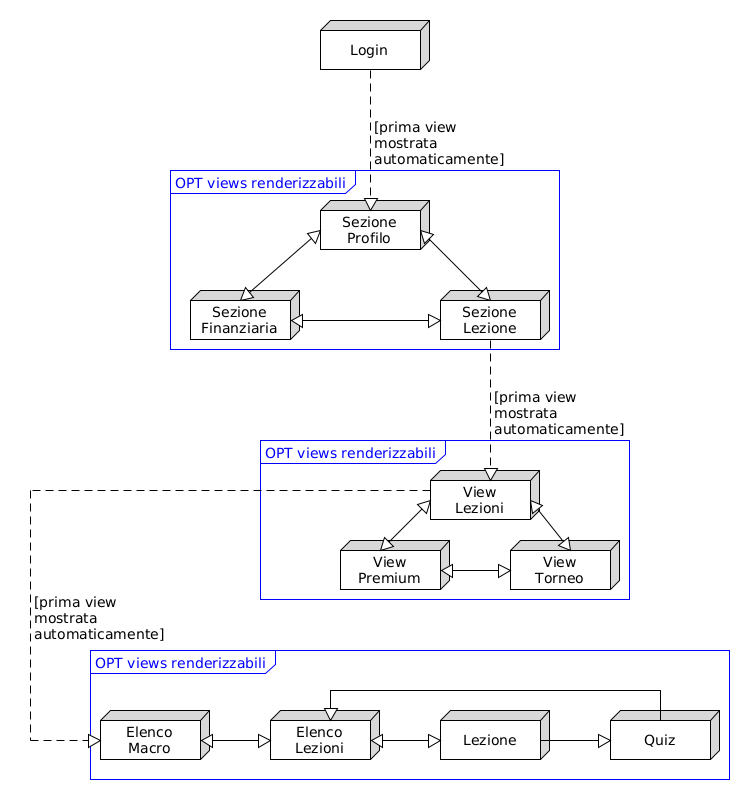
\includegraphics[scale=0.5]{pictures/schema_navigazione_schermate.png}}
    \hspace*{\dimexpr(\paperwidth-\textwidth)/15}
    \caption{Schema logico di navigazione delle schermate}
    \label{Schema logico di navigazione delle schermate}
\end{figure}



\begin{figure}[!htbp]
    \centering
    \makebox[0pt]{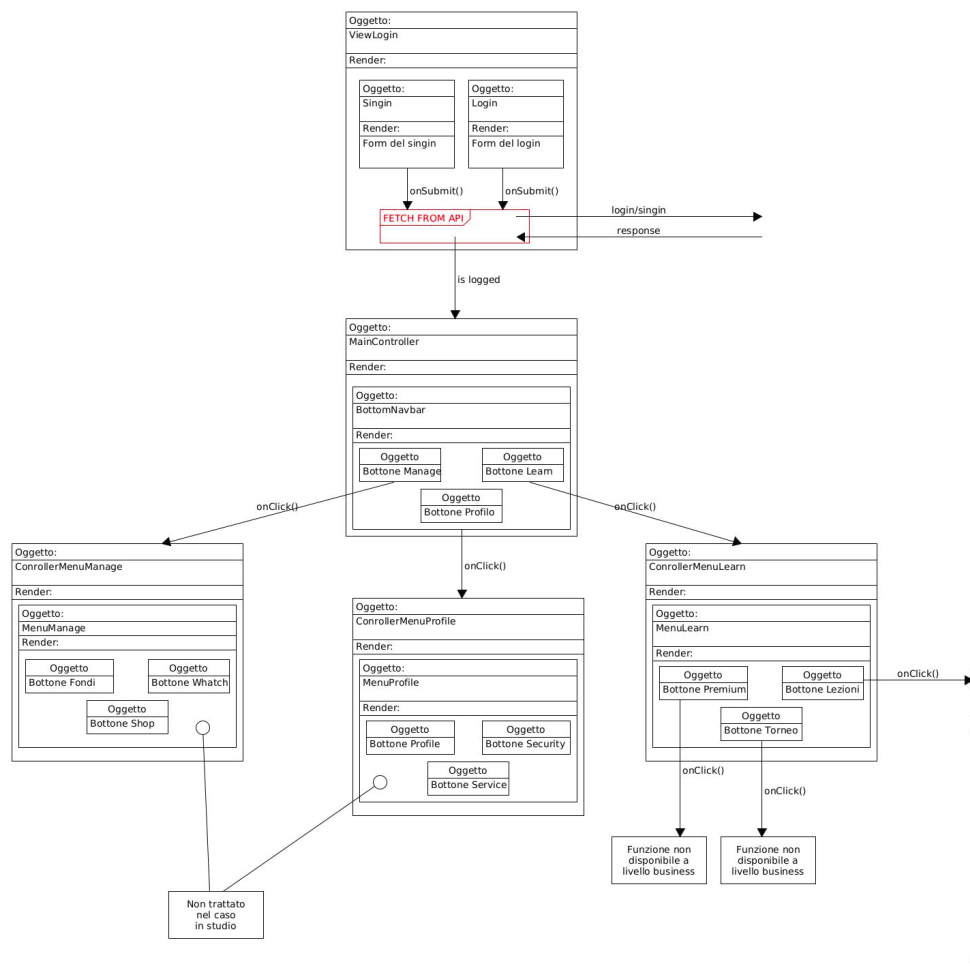
\includegraphics[scale=0.54, angle=270]{pictures/schema_generale_1.png}}
    \hspace*{\dimexpr(\paperwidth-\textwidth)/15}
    \caption{Schema della logica di funzionamento delle schermate pt.1}
    \label{Schema di funzionamento delle schermate pt.1}
\end{figure}


\begin{figure}[!htbp]
    \centering
    \makebox[0pt]{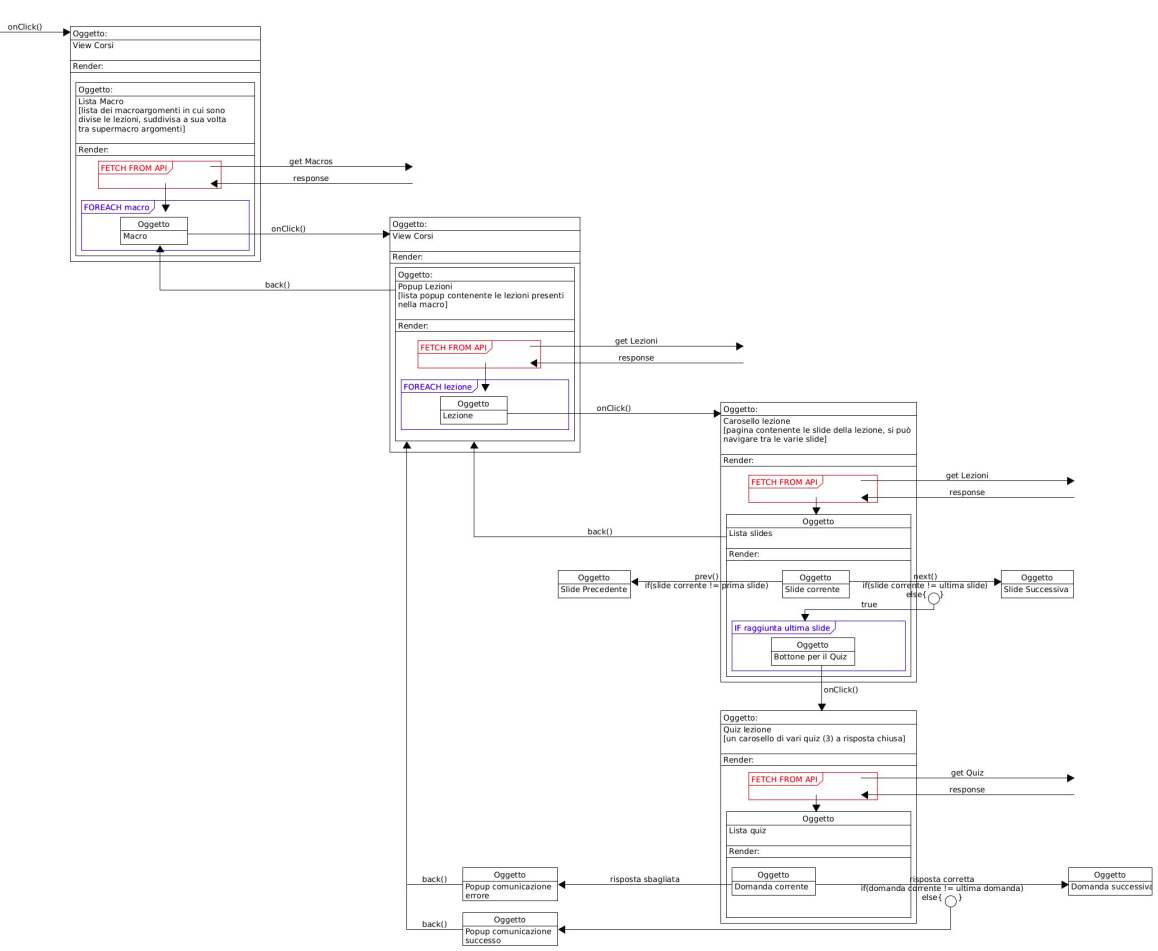
\includegraphics[scale=0.55, angle=270]{pictures/schema_generale_2.png}}
    \hspace*{\dimexpr(\paperwidth-\textwidth)/15}
    \caption{Schema della logica di funzionamento delle schermate pt.2}
    \label{Schema di funzionamento delle schermate pt.2}
\end{figure}






\newpage
\subsection{Backend}
Ho deciso di suddividere il backend in più api poiché essendo servizi piuttosto diversi tra loro voglio avere la possibilità di cambiare host, in base alla potenza o al livello di sicurezza che ritengo necessario per ogni singola api, senza dover aggiungere strati di complessità a quelle che non necessitano di particolare potenza o protezione.\\
L’api per recuperare i dati relativi alle lezioni deve semplicemente contattare un database e rispondere senza effettuare calcoli, non avrà quindi bisogno di particolare aumento di potenza di calcolo all’aumentare degli utenti. D’altra parte l’api per il calcolo del portafogli avrà bisogno di maggiore potenza all’aumentare degli utenti, poiché deve eseguire calcoli, e eventualmente essere posizionata sullo stesso server contenente un database di dati finanziari.\\
Altro caso in cui può essere necessaria una suddivisione potrebbe riguardare la sicurezza: le api per il calcolo dei portafogli e per recuperare le lezioni non hanno dei dati sensibili al loro interno, e se raggiunte o modificate da utenti malevoli il danno maggiore potrebbe essere l’utilizzo delle librerie o l’appropriarsi dei dati riguardanti le lezioni, cose tra l’altro disponibili gratuitamente con il download dell’app, quindi il danno più grave per il business potrebbe essere il blocco del loro corretto funzionamento.\\
Invece l’api da contattare per effettuare il login potrebbe esporre i dati sensibili e le credenziali di accesso degli utenti, che costituiscono una parte sensibile e di interesse per utenti malevoli, di conseguenza il livello di protezione dev’essere alto. Si può scegliere così di hostare l’api con i dati necessari al login su un server più sicuro, con un livello di crittografia maggiore e più protetto, cosa non necessaria per le api che recuperano esclusivamente dati non relativi all’utente, evitando così di aggiungere livelli di complessità non necessari che andrebbero a rallentarne il funzionamento.\\

\noindent
Confrontando le varie tecnologie disponibili ho selezionato Node.js per le api di login, lezioni e recupero dei dati finanziari principalmente per il suo funzionamento.\\
Node sfrutta l’interprete di javascript presente in Chrome, chiamato v8, che permette di risolvere le richieste in maniera non bloccante, tramite l’utilizzo di callback, migliorando la velocità del server. Ho utilizzato poi il framework Express per costruire un server con Node.\\
Invece per l’api per il calcolo dei portafogli ho preferito un server Python implementato tramite il microframework Flask. Questo framework leggero aggiunge solo gli elementi essenziali, evitando di dover riscrivere tanto codice “adapter” tra il server e l’utilizzo delle librerie. Per le librerie di calcolo dei portafogli ho scelto Python poiché permette uno sviluppo facile e veloce e ha molte librerie di calcolo complesso come “scipy” o “numpy” che evitano la riscrittura di complesse funzioni matematiche. Tuttavia Python non è particolarmente veloce e efficiente, perciò ho considerato l’opzione di dover riscrivere le librerie e l’api in un altro linguaggio per permettere una maggiore velocità dei calcoli.\\

\noindent
Il funzionamento generale delle API è molto simile, in generale il client invia una richiesta al server sull'ip pubblico con un certo path. Questa richiesta viene presa dal server web che la inoltra sulla porta corretta in base alla prima parte del path. Una volta arrivata all'api corretta il router, grazie alla seconda parte del path, richiama la funzione corrispondente. Questa funzione esegue i calcoli necessari, richiamando altre funzioni di libreria scritte da me, ne recupera il risultato e lo inoltra come risposta. In caso di errore invia un messaggio di errore di default.\\
La funzione richiamata dal router esegue delle operazioni preliminari prima di richiamare la funzione di libreria necessaria. Innanzitutto verifica che il database sia raggiungibile, se lo è richiama una funzione di login, per verificare che l'utente abbia i permessi per eseguire le operazioni. Se il login fallisce viene inviata una risposta al client che disconette l'utente, l'idea è che l'utente abbia una chiave per eseguire le operazioni, se questa chiave scade non può più eseguire operazioni, questo aumenta il livello di sicurezza poichè anche se viene intercettata una richiesta e decriptata, la chiave avrà solo un certo tempo per essere utilizzata. Se il login ha successo viene richiamata una funzione contenente le operazioni da eseguire e, una volta eseguite, viene inviata la risposta contenente i dati o l'esito positivo dell'operazione.

\subsubsection{Lista delle API}
Di seguito una lista con tutte le API e una loro breve descrizione.

\begin{enumerate}

\item[-] API di login    \begin{enumerate}
                            \item[-] \textbf{Linguaggio}: Node.js, Express
                            \item[-] \textbf{Richieste}: HTTP/POST
                            \item[-] \textbf{Descrizione}: API per effettuare login, singin e che gestisce il salvataggio e recupero dei dati personali relativi all'utente
                        \end{enumerate}
\item[-] API di finanza \begin{enumerate}
                            \item[-] \textbf{Linguaggio}:Node.js, Express
                            \item[-] \textbf{Richieste}: HTTP/POST
                            \item[-] \textbf{Descrizione}: API per effettuare tutte le operazioni riguardanti il lato finanziario quidni sia la gestione delle watchlists dell'utente, sia la gestione (acquisto o vendita) deli suoi portafogli
                        \end{enumerate}
\item[-] API delle lezioni \begin{enumerate}
                            \item[-] \textbf{Linguaggio}: Node.js, Express
                            \item[-] \textbf{Richieste}: HTTP/POST
                            \item[-] \textbf{Descrizione}: API che recupera i dati relativi alle lezioni e salva i progressi dell'utente
                        \end{enumerate}
\item[-] API del calcolatore \begin{enumerate}
                            \item[-] \textbf{Linguaggio}: Python, Flask
                            \item[-] \textbf{Richieste}: HTTP/POST
                            \item[-] \textbf{Descrizione}: API che calcola il portafoglio di ottimo in base al tipo di portafoglio richiesto e ai dati inviati
                        \end{enumerate}

\end{enumerate}


\newpage
\begin{figure}[!ht]
    \centering
    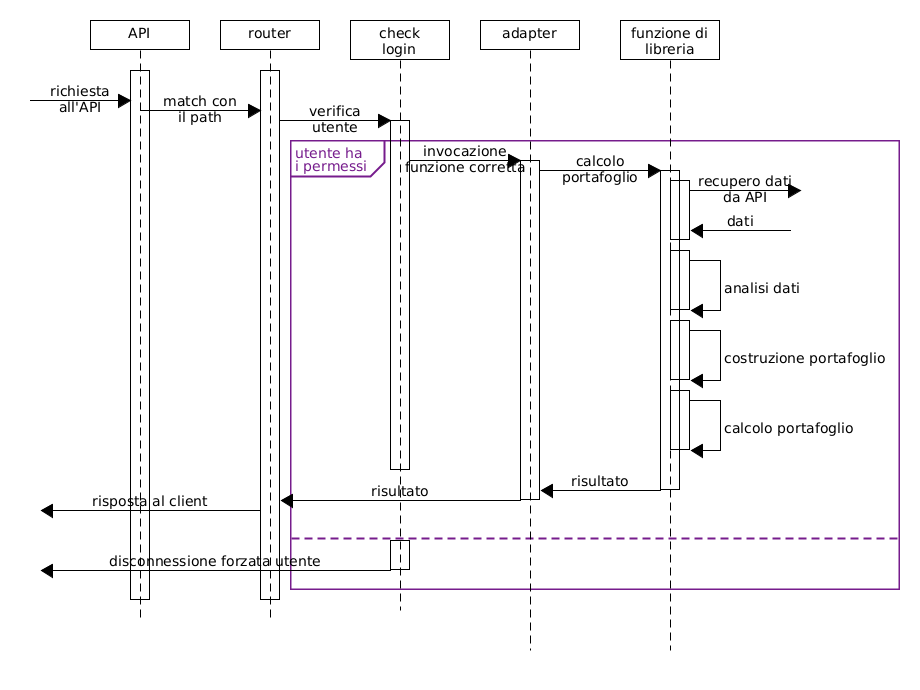
\includegraphics[scale=0.6, angle=270]{pictures/schema_generale_api_python.png}
    \caption{Schema di logica generale del funzionamento dell'API scritta in Python}
    \label{DSD dell'API Python}
\end{figure}

\begin{figure}[!ht]
    \centering
    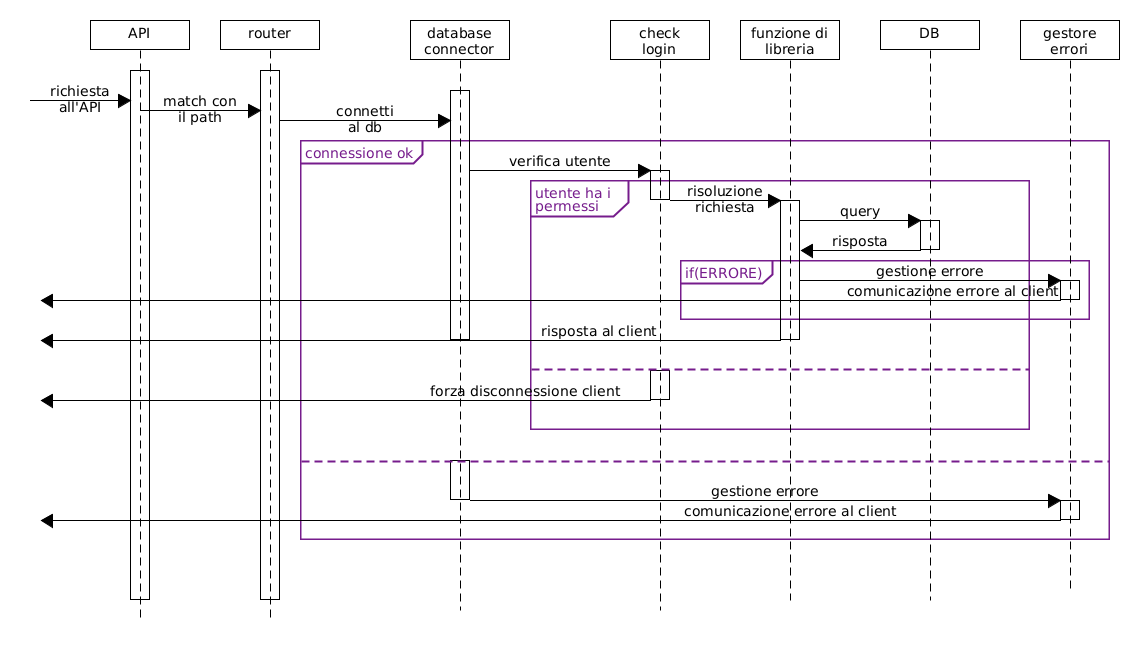
\includegraphics[scale=0.6, angle=270]{pictures/schema_generale_api_node.png}
    \caption{Schema di logica generale del funzionamento di un'API scritta in Node}
    \label{DSD delle API Node}
\end{figure}

\clearemptydoublepage
\chapter{Modello di Markowitz}
\section{Introduzione}
Questa introduzione è necessaria per spiegare il contesto in cui ci troviamo. Stiamo introducendo la Teoria di Markowitz, una teoria matematica per la costruzione di portafogli di titoli ottimizzati. Sono necessarie però un po’ di definizioni, a partire da quella di portafoglio di titoli.
Un portafoglio di titoli è un insieme di titoli finanziari, ovvero un insieme di azioni acquistabili nei vari possibili mercati finanziari. A ogni titolo presente nel portafoglio è associato un peso che è la percentuale di capitale a disposizione investito sul titolo, sul totale di capitale investito su tutti i titoli presenti nel portafoglio, quindi quanto ho investito su un cero titolo rispetto agli altri titoli presenti nel portafoglio.\\
Per ogni titolo sono importanti da considerare due parametri: il rischio e il rendimento.\\
Il rischio è legato alla varianza, la volatilità dei prezzi, ovvero quanto i valori storici si discostano dalla media, più un titolo è stabile (cresce e diminuisce poco) più è sicuro, più un titolo ha massimi e minimi distanti ( e quindi cresce e diminuisce tanto) più è incerto e ha rischio alto.\\
Il rendimento di un titolo è quanto il titolo ti può far guadagnare, più è alto il rendimento di un titolo, più si guadagna vendendolo. Il rendimento che generalmente si utilizza è detto lineare ed è il rendimento percentuale, ovvero il rendimento attuale in funzione del prezzo precedente e si calcola con la formula:\\
\formula{Rendimento percentuale}{
\[ rendimento = \frac{prezzo~attuale - prezzo~precedente}{prezzo~precedente}   \]
}
\noindent
Questa formula descrive proprio il concetto di rendimento, facendo un esempio pratico il "prezzo~precedente" potrebbe rappresentare il prezzo di acquisto, mentre il "prezzo~attuale" potrebbe rappresentare il prezzo di vendita, applicando la formula scopro in percentuale quanto ho guadagnato dall'operazione, ovvero il mio rendimento.\\
Markowitz considera al posto del rendimento, il rendimento atteso, cioè quanto l’investitore si aspetta di ottenere da uno o più titoli nel futuro. Ovviamente, poiché si tratta di un valore atteso, il rendimento realizzato potrebbe differire dal reale in quanto viene misurato riferendosi allo storico del titolo. Un criterio semplice potrebbe essere considerare il rendimento atteso pari al rendimento medio che il titolo ha registrato in passato. \\
Il rendimento medio è ottenuto tramite lo “stimatore della media”, che nel nostro caso è semplicemente la media aritmetica. La formula quindi è:\\
\formula{Rendimento medio}{\[ rendimento = \frac{prezzo_1 + prezzo_2 + ... + prezzo_n}{n} \]}
\noindent
Una raffinazione successiva potrebbe essere limitare l’analisi passata a un periodo minore di tutto lo storico e finanziariamente simile al periodo futuro in cui si vuole investire (ad esempio momenti di crisi o momenti di crescita). \\

\begin{Nota}
 Nota: Nella maggior parte dei casi non si potrà mai avere una stima della media affidabile, poiché per avere un valore affidabile servirebbero circa 90 anni di dati. Si può quindi scegliere di selezionare un periodo lungo probabilmente complessivamente poco simile al periodo di investimento o un periodo più corto e simile al periodo di investimento, ma con meno dati e quindi meno preciso.\\
\end{Nota}
\noindent
Tornando alla teoria di Markowitz, con portafoglio di ottimo si intende quella serie di pesi (ognuno legato a un titolo presente nel portafoglio) per cui complessivamente il portafoglio avrà il massimo rendimento atteso e il minimo rischio, ovvero la minima varianza.\\
Abbiamo quindi ora i concetti base per spiegare la teoria di Markowitz.

\vspace{1cm}
\section{Teoria del modello di Markowitz}

La teoria di Markowitz prende il nome dal suo ideatore, Henry Markowitz (Chicago, 24 agosto 1927)  economista statunitense che vinse nel 1990 il premio Nobel per l’economia. 
Markowitz sosteneva che per costruire un portafoglio occorre individuare titoli la cui combinazione minimizzi il rischio e massimizzi il rendimento; per fare ciò fu il primo a introdurre il concetto di correlazione fra i titoli.
Oltre al rischio del singolo titolo, è importante considerare il rischio di un portafoglio composto da due o più titoli, il quale dipende dalla correlazione esistente tra essi. Se non esiste alcuna correlazione tra i diversi titoli, il rischio di portafoglio sarebbe analogo a quello dei singoli titoli, questo perché non vi è covarianza, come si vede dalla formula del rischio del portafoglio.

\formula{Covarianza}{\[ covarianza = \sum{\frac{(x_i - media(x)) \ast (y_i - media(y))}{n-1}} \]}
\begin{Nota}
 Nota: n $\rightarrow$ numero dei dati\\
\end{Nota}

\noindent
Considerando due titoli e il loro coefficiente di correlazione, se questo è positivo o negativo la crescita del rendimento di un titolo corrisponde l’aumento o decremento del rendimento del secondo titolo. Si deduce che nel caso di andamenti contrapposti dei rendimenti dei titoli – ovvero il concetto di diversificazione – il rischio globale di un portafoglio si riduce perché si va a ridurre il rischio “idiosincatico” a zero (ovvero il rischio legato all’andamento del singolo titolo, annullabile diversificando), rimane intatto però il rischio “di mercato” (ovvero il rischio sistematico che non può essere ridotto poiché dato dall’incertezzza del mercato data da eventi esterni ), che non può essere eliminato in nessun caso poiché intrinseco al mercato stesso. In parole povere se riesco a inserire titoli ben correlati tra di loro il rischio globale diminuisce poiché se un titolo scende, e quindi perde valore, i titoli a lui correlati salgono, e quindi acquistano valore, compensandosi.
Il modello di Markowitz serve a tracciare una curva che descrive tutte le possibili combinazioni di titoli all’interno del portafoglio. Questa curva è chiamata “frontiera efficiente”  poiché mostra quale è la volatilità minima associata a ogni livello di  rendimento atteso.\\
Ogni punto della curva è un possibile combinazione del portafoglio e andando a vedere le coordinate di ogni punto abbiamo sulla x la varianza e sulla y il rendimento.

\begin{figure}[!ht]
    \centering
    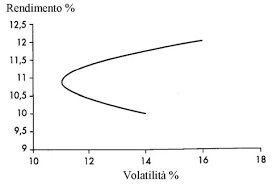
\includegraphics[scale=1.2]{pictures/grafico_markowitz.png}
    \caption{Curva di Markowitz}
    \label{Curva di Markowitz}
\end{figure}

\noindent
In questa curva abbiamo 3 parti di interesse:
\begin{enumerate}
\item[-] La prima è la parte di curva che tende verso il basso e verso destra, questa parte è da ignorare, poiché, come si vede dal grafico il rendimento di un portafoglio diminuisce all’aumentare della volatilità, nessun investitore investirebbe in un tale portafoglio (e quindi in una tale combinazione di titoli. Inoltre guardando il grafico si nota che a parità di volatilità c’è un maggiore valore di rendimento, ciò ci porta alla seconda parte interessante.
\item[-] La seconda parte della curva di interesse è la parte che tende verso l’alto e verso destra, è detta “frontiera efficiente” poiché descrive solo i portafogli il cui investimento può essere interessante per un investitore che desidera massimizzare il rendimento, anche a costo di aumentare la volatilità. Questa parte comprende quindi solo i portafogli che per ogni livello di volatilità offrono il rendimento più elevato possibile.
\item[-] La terza è un punto, è la combinazione che compone il “portafoglio a varianza minima globale” (o “portafoglio a volatilità minima globale”), graficamente è il punto più a sinistra nella curva e descrive il portafoglio con il rischio minimo.
\end{enumerate}


\noindent
Note matematiche:
\begin{enumerate}
    \item[-] A noi interessa la curva, ma in realtà i punti che compongono l’area interna alla curva sono anch’essi delle combinazioni di titoli del portafogli, ma non sono quelle efficienti a parità di volatilità. L’area interna è chiamata “opportunity set”.
    \item[-] Nella realtà la curva è considerata finita, ma nella teoria matematica si può espandere verso l’alto all’infinito. Chiaramente questo implica che il rendimento e il rischio. assumeranno valori molto alti. Per eguagliare un rendimento molto altro l’investitore potrà vendere allo scoperto, assumendo una posizione di short contro il titolo, a questo però corrisponderà un rischio >1, ciò significa che se perde, perderà più capitale di quello che ha investito.
\end{enumerate}

\noindent
Da questa teoria matematica si parte per risolvere il problema dell’ottimizzazione, poiché fissato un certo rendimento desiderato basterà prendere sulla curva il punto corrispondente a quel rendimento (si ricorda che a ogni punto corrisponde una combinazione di pesi, prendere un punto vuol quindi dire utilizzare quei pesi).

\vspace{1cm}
\section{Metodo “a mano”}

Per utilizzare la teoria di Markowitz si parte da un vettore contenete i rendimenti medi per ogni titolo che si vuole inserire nel portafoglio e una matrice di covarianze, in cui ogni posizione [i,j] conterrà la covarianza tra il titolo i e il titolo j, si noti che la diagonale contiene le varianze dei singoli titoli, essendo che covarianza(titolo i, titolo i) == varianza(titolo i). Nell’utilizzo al computer questi dati ce li calcoliamo, negli esercizi svolti a mano generalmente questi due dati (vettore medie e matrice covarianze) vengono dati dal problema.\\
Imposto poi il sistema. Si tratta di un sistema di ottimo vincolato con una funzione obbiettivo convessa, che è la lagrangiana:

\formula{Lagnangiada~di~Markowitz}{
\[ L(\lambda_1, \lambda_2,x) = x^TVx + \lambda_1 (m - \mu^Tx) + \lambda_2 (1- e^Tx) \]
}
\noindent
Risolvendo il sistema riesco cosi a ottenere la curva (che è una iperbole) in funzione di a, b e c descritta dalla seguente formula:
\formula{Curva~di~Markowitz}{\[\sigma = \sqrt{\frac{cm^2-2bm+a}{ac-b^2}}\]}

Con a, b, c:
\noindent
\formula{Parametro a}{\[ a = \mu^T * V^{-1} * \mu\]}
\formula{Parametro b}{\[b = \mu^T * V^{-1} * e \]}
\formula{Parametro c}{\[c = e^T * V^{-1} * e \]}



\begin{Nota}
    Didascalia:
    \begin{enumerate}
        \item[-] V $\rightarrow$ matrice delle covarianze
        \item[-] $\mu \rightarrow$ vettore delle medie dei titoli
        \item[-] e $\rightarrow$ vettore sommatoria\\
    \end{enumerate}

    Reminder delle operazioni:
    \begin{enumerate}
        \item[-] $x^T \rightarrow$ x trasposto
        \item[-] $x^{-1} \rightarrow$ x inverso
    \end{enumerate}
\end{Nota}



\noindent
Questa formula descrive la curva del rischio in funzione di m, ovvero il rendimento atteso.\\
Da questa formula parto per riscrivere una seconda formula per trovare la x,ovvero il vettore dei pesi, in funzione di m, ovvero il rendimento atteso.


\formula{Vettore~dei~pesi}{\[ x = \frac{((m*c-b) * \mu^T * V^{-1} * (a-m*b)*e^T*V^{-1})^T}{ a*c-b^2 }\]}



\noindent
Impostando quindi in questa formula una certa m a scelta e i valori di a,b e c calcolati con le formule precedentemente presentate è possibile trovare sulla curva il punto che possiede il rendimento corrispondente e un certo vettore dei pesi che a noi interessa.\\
Si noti che vi è un certo rendimento minimo, infatti prendendo solo il ramo dell’iperbole maggiore del punto detto “portafoglio a varianza minima globale” non sarà possibile ottenere un rendimento minore del rendimento associato a questo punto. Bisogna così calcolarsi m*, ovvero il rendimento del “portafoglio a varianza minima globale”, e verificare che il rendimento atteso sia maggiore di m*  

\vspace{1cm}
\section{Dalla penna al computer}
\subsection{processo di sviluppo dello pseudocodice}
Visto come si esegue questo calcolo a mano si tenta di tradurre questa serie di passaggi in algoritmo.
Innanzitutto a noi interessa x, ovvero il vettore dei pesi, calcolato con\\
\[ x = \frac{((m*c-b) * \mu^T * V^{-1} * (a-m*b)*e^T*V^{-1})^T}{ a*c-b^2 }   
\]\\
\noindent
per risolvere questa formula abbiamo bisogno di m, a, b, c, $\mu$ (array medie titoli), V (matrice covarianza) e e(vettore sommatoria).\\
M viene richiesta come input quindi ce l’abbiamo. Abbiamo bisogno di a,b,c che, dalle formule scritte sopra, per essere calcolati hanno bisogno di mu e V come input.\\
V e $\mu$ non ce li abbiamo e per ricavarli utilizziamo i dati grezzi. Partiamo quindi da calcolare $\mu$ e V a partire dai valori di chiusura medi settimanali. \\
I valori di chiusura medi settimanali si recuperano da delle API che prendono i dati da dei database (ad esempio tramite una api di yahoo finance). Sono la media dei prezzi di una azione al momento della chiusura del mercato, prendendo il prezzo in ogni giorno nell’arco di una settimana e facendone la media si ottiene il valore di chiusura medio di una settimana per una certa azione.\\ 
Noi quindi per calcolare i dati necessari impostiamo un certo periodo di tempo in cui verrà fatta l’analisi e andiamo a recuperare per i titoli selezionati i valori di chiusura media di ogni settimana. Si ricorda che il periodo passato analizzato dovrebbe essere simile al periodo futuro in cui verrà fatto l’investimento.\\

\noindent
Ottenuta questa grande matrice contenente i titoli e i relativi prezzi di chiusura settimanali andiamo a calcolare $\mu$ e V.\\ 
Per calcolare $\mu$ facciamo la media aritmetica dei prezzi per ogni titolo, otteniamo così un’array lungo quanto la quantità di titoli contenente in ogni posizione la media di un certo tiolo. \\
Per calcolare V si utilizza la varianza e la covarianza. La posizione \code{V[i,j]} è infatti data dalla covarianza tra \code{titolo[i]} e \code{titolo[j]} presenti nella matrice delle chiusure settimanali, quindi la funzione \code{covarianza()} prende in input due array, che devono essere della stessa dimensione, contenenti i prezzi di chiusura settimanali e ne calcola un numero, che è la covarianza. Da notare che la covarianza tra \code{titolo[i]} e \code{titolo[i]} (quindi la covarianza tra lo stesso titolo) è uguale alla varianza di quel titolo. Otteniamo quindi una matrice che ha sulla diagonale (dove i==j) ha le varianze dei singoli titoli e nelle altre posizioni tutte le covarianze, da notare che è una matrice che si può specchiare sulla diagonale poiché la covarianza tra i e j è uguale alla covarianza tra j e i.\\

\noindent
Adesso possiamo calcolare a, b e c con le formule:

\noindent
\[a = \mu^T * V^{-1} * \mu\] 
\[b = \mu^T * V^{-1} * e \]
\[c = e^T * V^{-1} * e \]

\noindent
Può essere necessario alla comprensione spiegare cosa sono il vettore sommatoria e una lista trasposta. Una generica matrice trasposta è una matrice in cui le righe vengono sostituite dalle colonne e viceversa, quindi l’effetto di trasposizione su una lista colonna (ovvero un array) mi farà ottenere una matrice con tante colonne quante righe del vettore e ogni colonna conterrà un solo elemento. \\
Il vettore sommatoria è un vettore composto da solo 1, è detto sommatoria poiché se moltiplicato (o meglio post-moltiplicato) per un altro vettore il risultato che si ottiene è la sommatoria del primo vettore, si ricorda che la moltiplicazione tra vettori, il primo verticale e l’altro orizzontale, è data dalla sommatoria delle moltiplicazioni tra i valori nella stessa posizione dei due vettori.\\

\noindent
Ora che abbiamo $\mu$, V, a,b, e c calcoliamo m* per verificare che l’m richiesto sia maggiore, e quindi il calcolo sia effettuabile.\\
Con questa formula possiamo calcolare m*:
\formula{Parametro m*}{\[ m* = \frac{-B}{2*C} \]}
con:
\formula{Parametro B}{\[ B = \frac{2*b}{a*c-b^2}\]}
\formula{Parametro C}{\[C = \frac{c}{a*c-b^2}\]}
\noindent
Se m>m* allora si può procedere a calcolare la x con la formula già data in precedenza
\[ x = \frac{((m*c-b) * \mu^T * V^{-1} * (a-m*b)*e^T*V^{-1})^T}{ a*c-b^2 }\]
\\
\noindent
Si ottiene così un vettore contenente i pesi di ogni titolo. Da notare che questo vettore rappresenta la percentuale di capitale da investire in ogni titolo, la sommatoria del vettore quindi deve essere teoricamente 1, in realtà però sarà circa 1 (può non essere esattamente uno a causa dell’approssimazione). Se il peso relativo al titolo è positivo bisognerà acquistare quel titolo utilizzando una percentuale del capitale da investire corrispondente al peso, se il peso è negativo bisognerà vendere allo scoperto quel titolo in quantità pari alla percentuale del capitale corrispondente al peso.

\newpage
\subsection{Pseudocodice}


\begin{minted}{java}


//lista contenente i nomi dei titoli che 
//si desidera inserire nel portafoglio
title_list = [ "title1", "title2", "title3" ] 

//dati grezzi dei titoli
raw_title_matrix = get_rew_datas(title_list)

//si calcola l'array delle medie
a_mean = [] //array delle medie
foreach( title in raw_prices_matrix ){
	a_mean[title] = mean(raw_prices_matrix [title])
}

//calcolo la matrice di covarianza
matrix_covar = [] //matrice covarianza
for( i in length(title_list)){
	row = [] //lista in cui si accumulano i risultati
	for (j in length(title_list)){
		if (i==j){
			row.append( varianza(raw_title_matrix[i] )
		}else{
			row.append(covarianza(raw_title_matrix[i],
			                        raw_title_matrix[j] )
		}	
	}
	matrix_covar.append(row)
}

//calcolo i parametri utili
a = find_a(a_mean, matrix_covar)
b = find_b(a_mean, matrix_covar)
c = find_c(matrix_covar)
B = find_B(a,b,c)
C = find_C(a,b,c)

//calcolo m*
m* = find_m*(B,C)

//verifico se m richiesto è valido
if(m*>m){
	return null //impossibile calcolare il risultato
}

//qua m è accettabile per il calcolo
 
\end{minted}
 \begin{Nota}
 A questo punto applico la formula: $x = \frac{((m*c-b) * \mu^T * V^{-1} * (a-m*b)*e^T*V^{-1})^T}{ a*c-b^2 }$
 \end{Nota}
\begin{minted}{java}

parz_1= mul_array_matrix( mul_scalar_vector((m*c-b), traspose(mu)),
                                inverse(V))
parz_2= mul_array_matrix( mul_scalar_vector((a-m*b), traspose(vect_sum)),
                                inverse(V))  
num = sum_vectors( traspose(parz_1), parz_2)
num_traspose = traspose(num) 
denom = (a*c)-(b*b) 

x = div_array_scalar( num_traspose, denom )
// a questo punto x è una lista contenente tutti i pesi

//da qua si fanno delle operazioni di controllo e formattazione

//controllo che la sommatoria dell’array sia =1
if(summation(x) not 1){
    return null
}else{
//ritorno l'array contenente i pesi
    return x
}
    
\end{minted}


\clearemptydoublepage




%%%% TAIL OF THE DOCUMENT
\chapter{Conclusioni}
In conclusione lo stage non si è concentrato su una singola parte in maniera dettagliata e approfondita, bensì su una ampia gamma di strumenti e linguaggi.\\
Ho lavorato sia allo sviluppo del frontend in React, sia allo sviluppo del backend in Node e Python ma oltre lo studio di nuovi linguaggi, framework e paradigmi di programmazione la parte che ho trovato più formativa (e stimolante) è stato impostare tutto il sistema per poter distribuire l'applicazione. Non ho trattato questa parte nella tesi poichè non la ritengo particolarmente interessante e ci ho dedicato solo una piccola parte del tempo (non è complicato o lungo settare un server web), eppure mi ha costretto a lavorare con strumenti che non conoscevo e a studiare personalmente una soluzione ottimale per poter far funzionare tutto al meglio.\\

\noindent
Un altro punnto che voglio trattare è il presente e il futuro dell'applicazione. Attualmente siamo andati avanti nello sviluppo da ciò che ho inserito nello stage. Per quanto riguarda la società abbiamo in programma, io e il mio socio, di costituirci come startup (srl innovativa) a breve, una volta costituiti affideremo lo sviluppo frontend mancante a una socità estenra per accellerare il processo di sviluppo. A livello di backend sto finendo di sviluppare l'api Node con la parte riguardante l'acquisto e la vendita di portafogli. L'obiettivo attuale è riuscire a lanciare per inizio gennaio 2022 una beta su un campione di medie dimensioni di studenti per poter acquisire importanti dati su utilizzo e usability che ci daranno una corretta indicazione sulla direzione che dovrebbe prendere lo sviluppo e ci permetteranno di definire ulteriormente il modello di business. 



%bibliography
\chapter*{Bibliografia}

Bibliografia:
\begin{enumerate}
    \item [-] Andrea Beltratti, \textit{Investimenti finanziari} , editore EGEA, 2020
\end{enumerate}

\noindent
\newline
Sitografia:
\begin{enumerate}
    \item [-] Documentazione ufficiale \textit{Node.js}, https://nodejs.org/it/
    \item [-] Documentazione ufficiale framework \textit{Express}, https://expressjs.com/it/
    \item [-] Documentazione ufficiale \textit{Python}, https://www.python.org/
    \item [-] Documentazione ufficiale framework \textit{Flask}, https://flask.palletsprojects.com/en/2.0.x/
    \item [-] \textit{Wikipedia}, https://it.wikipedia.org/
    \item [-] \textit{Stackoverflow}, https://stackoverflow.com/
\end{enumerate}


\end{document}
